
Die Informatik umfasst eine Vielzahl unterschiedlicher Fachgebiete mit teils stark variierenden Schwerpunkten. 
Dazu zählen unter anderem die Web- und Anwendungsentwicklung sowie der Bereich der IT-Sicherheit und viele weitere Disziplinen. 
Im Rahmen dieser Arbeit liegt der Fokus auf dem speziellen Teilbereich der Embedded-Softwareentwicklung.

In diesem Kapitel werden die grundlegenden fachlichen und technischen Konzepte vermittelt, die zum Verständnis der weiteren Inhalte erforderlich sind
% Ablauf des Kapitels
Zu Beginn wird eine Einführung in das Themenfeld der Embedded-Softwareentwicklung gegeben, um ein klares Verständnis dafür zu schaffen, welche Unterschiede diesen Bereich kennzeichnen und wie er sich von anderen Teilgebieten der Informatik unterscheidet.
Darauffolgend werden zentrale Begriffe und Konzepte erläutert, die in der Embedded-Entwicklung eine signifikante Rolle spielen, wie beispielsweise Register, Ports, Peripherieansteuerung und hardwarenahe Programmierung.
Darüber hinaus wird technisches Hintergrundwissen vermittelt, das für das Verständnis der späteren Implementierungsschritte und der Architekturentscheidungen von Relevanz ist.

Das Ziel dieses Kapitels besteht darin, eine solide Wissensbasis zu schaffen, auf der die Analyse bestehender Lösungen sowie die Entwicklung einer eigenen Treiber-API aufbauen können.

\section{Embedded Systems}
Bevor auf die Entwicklung eingebetteter Systeme eingegangen werden kann, ist zunächst zu klären, worum es sich bei diesen Systemen handelt.
Der Begriff \emph{''Embedded System''} (deutsch: eingebettetes System) bezeichnet ein Computersystem, das aus Hardware und Software besteht und fest in einen übergeordneten technischen Kontext integriert ist. 
Typischerweise handelt es sich dabei um Maschinen, Geräte oder Anlagen, in denen das eingebettete System spezifische Steuerungs-, Regelungs- oder Datenverarbeitungsaufgaben übernimmt.
Ein wesentliches Merkmal eingebetteter Systeme besteht darin, dass sie nicht als eigenständige Recheneinheiten agieren, sondern als integraler Bestandteil eines übergeordneten Gesamtsystems dienen.
In der Regel operieren sie im Hintergrund und sind nicht direkt mit den Benutzern verbunden. In einigen Fällen erfolgt die Interaktion automatisch, in anderen durch Eingaben des Nutzers.

\paragraph{Definition:}
Ein Embedded System ist ein spezialisiertes, in sich geschlossenes Computersystem, das für eine klar definierte Aufgabe innerhalb eines übergeordneten technischen Systems konzipiert wurde.

\vspace{6 mm}

Die Entwicklung von Software für eingebettete Systeme ist mit besonderen Anforderungen verbunden, die sich signifikant von denen unterscheiden, die etwa in der Web- oder Anwendungsentwicklung üblich sind.
Es ist von besonderer Bedeutung, hardwarenahe Aspekte zu berücksichtigen, da die Software unmittelbar mit der zugrunde liegenden Mikrocontroller-Hardware interagiert.
Ein zentraler Aspekt dabei ist die Integration geeigneter Treiber für die jeweilige Mikrocontroller-Architektur.
Die betreffenden Treiber beinhalten Funktionen, welche den Zugriff auf die Hardware mittels sogenannter Register erlauben.
Register sind spezifische Speicherbereiche innerhalb des Mikrocontrollers, welche eine unmittelbare Manipulation des Hardware-Verhaltens ermöglichen.
Durch das gezielte Setzen oder Auslesen einzelner Bits in diesen Registern ist es möglich, beispielsweise Sensorwerte zu erfassen (z. B. das Drücken eines Tasters) oder Ausgaben zu erzeugen (z. B. das Anzeigen eines Textes auf einem Display).



\section{Begriffe und Erklärungen}

\subsection*{Microprozessor Unit (MPU)}
Ein Mikroprozessor ist ein vollständig auf einem einzigen integrierten Schaltkreis (Chip) realisierter Prozessor.
Der Prozessor ist die zentrale Recheneinheit eines Computersystems.
Seine Funktion umfasst die Ausführung von Befehlen sowie die Steuerung des Datenflusses innerhalb des Systems. 
Ein Mikroprozessor beinhaltet in der Regel Komponenten wie das Rechenwerk (ALU), Register, Steuerwerk und gegebenenfalls Caches, jedoch keine Peripheriefunktionen wie Speicher oder Schnittstellen. 
Diese müssen extern angebunden werden.
Der Begriff "Mikrocomputer" wird verwendet, um ein auf Basis eines Mikroprozessors aufgebautes Gesamtsystem zu definieren. 
Derartige Systeme sind in klassischen Personal Computern, Laptops oder Servern häufig anzutreffen.
In diesen Geräten wird der Mikroprozessor mit externem RAM, ROM, I/O-Komponenten und weiteren Funktionseinheiten kombiniert.

Demgegenüber ist der Mikrocontroller für spezifische Steuerungsaufgaben mit integrierten Peripheriefunktionen konzipiert. 
Der Mikroprozessor findet dagegen meist in leistungsfähigen, aber nicht auf eine konkrete Aufgabe spezialisierten Systemen Anwendung. 
Insbesondere für allgemeine Rechenaufgaben, komplexe Betriebssysteme sowie Anwendungen mit hohem Ressourcenbedarf erweist sich dieser Prozessor als geeignet.

\subsection*{Microcontroller Unit (MCU)}
Ein Mikrocontroller ist ein vollständig auf einem einzigen Chip realisierter Mikrocomputer, der neben dem eigentlichen Prozessor (CPU) auch sämtliche für den Betrieb notwendigen Komponenten integriert. 
Zu den Komponenten eines solchen Systems zählen in der Regel Programmspeicher (Flash), Datenspeicher (RAM), digitale Ein- und Ausgänge (GPIO), Timer, Kommunikationsschnittstellen (wie UART, SPI, I$^2$C, CAN) sowie in vielen Fällen analoge Peripheriekomponenten wie A/D-Wandler oder PWM-Einheiten.

Mikrocontroller werden für spezifische Steuerungs- und Regelungsaufgaben konzipiert und finden typischerweise Anwendung in eingebetteten Systemen, wie beispielsweise Haushaltsgeräten, Fahrzeugsteuerungen, Industrieanlagen oder IoT-Geräten. 
Die Geräte zeichnen sich durch einen geringen Energieverbrauch, eine kompakte Bauform, niedrige Kosten und eine direkte Hardwareansteuerung aus. 
Im Vergleich zu Mikroprozessoren sind für den Grundbetrieb von Mikrocontrollern keine externen Komponenten erforderlich, was besonders kompakte und zuverlässige Systemlösungen ermöglicht.


%\subsection*{Hardware Architektur}
%- CISC vs. RISC
%
%- Cortex Familie


\subsection*{Register}
Register sind kleine, besonders schnell zugängliche Speicherzellen, die direkt im Prozessor untergebracht sind. 
Im Gegensatz zu anderen Speicherformen, wie etwa RAM oder Flash, zeichnen sich Register durch extrem kurze Zugriffszeiten aus. 
Dies ist darauf zurückzuführen, dass sie Teil des zentralen Rechenwerks sind. 
Die Nähe zur Recheneinheit ist dabei von entscheidender Bedeutung, insbesondere für grundlegende Operationen wie das Zwischenspeichern von Werten, Adressen oder Zustandsinformationen während der Programmausführung.

Im Kontext eingebetteter Systeme und insbesondere bei der Treiberentwicklung spielen sogenannte speicherabbildende Register (Memory-Mapped Registers) eine zentrale Rolle. 
Diese sind Teil der Hardwareperipherie (wie GPIO, SPI oder UART) und über spezifische Speicheradressen ansprechbar. 
Durch das Schreiben in oder Lesen aus solchen Registern können spezifische Hardwarefunktionen aktiviert, deaktiviert oder abgefragt werden.

Ein konkretes Beispiel ist ein GPIO-Ausgangsregister: Wird ein bestimmtes Bit darin gesetzt, liegt am zugeordneten Pin ein logisches High-Signal an. 
Die exakte Kenntnis über die Position und Signifikanz dieser Bits ist essenziell für die direkte Hardwareprogrammierung und die korrekte Umsetzung von Treibern.
\\
Register werden somit nicht nur für die interne Funktionsweise des Prozessors relevant, sondern bilden auch die Schnittstelle zwischen Software und Hardware. Es sei darauf hingewiesen, dass diese Elemente die Konfiguration, Steuerung und das Auslesen externer Peripheriekomponenten ermöglichen und somit das zentrale Element bei der Low-Level-Programmierung darstellen.

\subsection*{Peripherie}
Unter dem Begriff der \emph{Peripherie} versteht man im Kontext der Embedded-Softwareentwicklung sämtliche Ein- und Ausgabeschnittstellen, die eine Interaktion des Mikrocontrollers mit seiner Umwelt ermöglichen.

% TODO: Parallel/Seriell; synchron/asynchron; für alle nochmal drüber gehen
\subsubsection*{GPIO}
Der Begriff \emph{General Purpose Input/Output} (GPIO) bezeichnet universelle digitale Ein- und Ausgänge, die sich durch eine hohe Flexibilität für verschiedenste Aufgaben auszeichnen.
Sie ermöglichen es dem Mikrocontroller zum Beispiel, digitale Signale zu lesen (Input) oder zu erzeugen (Output), um etwa Taster auszuwerten oder LEDs anzusteuern. 
GPIOs stellen somit die einfachste Form der Peripherieanbindung dar.

\subsubsection*{SPI}
Die Schnittstellen des \emph{Serial Peripheral Interface} (SPI) ist ein synchrones, serielles Kommunikationsprotokoll, das insbesondere für die schnelle Datenübertragung zwischen einem Master- und mehreren Slave-Geräten eingesetzt wird. 
Zu den typischen Einsatzgebieten zählen die Anbindung von Sensoren, Displays oder Speichern. 
SPI zeichnet sich durch eine hohe Übertragungsgeschwindigkeit und einfache Implementierung aus.

\subsubsection*{UART}
Der \emph{Universal Asynchronous Receiver Transmitter} (UART) ist ein asynchrones Kommunikationsprotokoll, das insbesondere für die serielle Punkt-zu-Punkt-Kommunikation eingesetzt wird. 
Das Gerät eignet sich für verschiedene Anwendungsbereiche, darunter das Debugging, der Anschluss von GPS-Modulen sowie die Kommunikation mit Computern über USB-zu-Seriell-Wandler. 
UART zeichnet sich durch eine hohe Verbreitung aus und erfordert im Gegensatz zu SPI oder I2C keine zusätzliche Taktleitung.

\subsubsection*{CAN}
Das \emph{Controller Area Network} (CAN) ist ein robustes, asynchrones Bussystem, das insbesondere in der Automobilindustrie eine weite Verbreitung findet. 
Es ermöglicht eine zuverlässige Kommunikation zwischen mehreren Steuergeräten (Nodes), auch unter schwierigen elektromagnetischen Bedingungen. 
Der Einsatz von CAN in sicherheitskritischen Anwendungen beruht auf zwei wesentlichen Eigenschaften: 
\begin{itemize}
	\item der prioritätsbasierten Arbitrierung
	\item der integrierten Fehlererkennung
\end{itemize}
 
 Diese Eigenschaften gewährleisten eine hohe Ausfallsicherheit.

%\subsection*{Hardware Abstraction Layer (HAL)}
%
%- abstrahiert den Anwendungscode auf Hardwarenahen Code.
%
%- beinhaltet Funktionen um die Register des Spezifischen MCU anzusprechen/zu steuern.
%
%- für STM32 Hardwareboards

% TODO: CMSIS nochmal überarbeiten
\subsection*{Common Microcontroller Software Interface Standard (CMSIS)}
Der \emph{Common Microcontroller Software Interface Standard} stellt einen von Arm entwickelten Industriestandard dar, der eine einheitliche Softwarearchitektur für Mikrocontroller auf Basis der Arm-Cortex-Prozessorfamilie bereitstellt.
Der Begriff "CMSIS" bezeichnet eine Sammlung von Schnittstellen, Softwarekomponenten, Header-Dateien, Entwicklungswerkzeugen und Workflows.
 Die Sammlung soll die Portabilität, Wiederverwendbarkeit und Effizienz im Bereich der Softwareentwicklung für eingebettete Systeme steigern.
Das Ziel von CMSIS besteht darin, eine konsistente und herstellerübergreifende Abstraktion der zugrunde liegenden Hardware bereitzustellen, um die Integration verschiedener Entwicklungswerkzeuge und Bibliotheken zu erleichtern.
Die Standardisierung ermöglicht es Entwicklerinnen und Entwicklern, auf einheitliche Weise auf Prozessorfunktionen, Peripherie und Betriebssystemfunktionen zuzugreifen, unabhängig vom konkreten Mikrocontrollerhersteller.

Die Sammlung ist in mehrere Module unterteilt, darunter:
\begin{itemize}
	\item \textbf{CMSIS-Core:} Definieret standardisierter Zugriffsmöglichkeiten auf CPU-Register und Systemfunktionen sowie auf Start- und Systeminitialisierungscode.
	\item \textbf{CMSIS-Driver:} Definiert eine einheitliche Schnittstelle für Peripherietreiber wie UART, SPI oder I$^2$C.
	\item \textbf{CMSIS-DSP:} Stellt eine optimierte Lösung für die digitale Signalverarbeitung bereit und unterstützt sowohl Vektor- als auch Matrizenoperationen.
	\item \textbf{CMSIS-RTOS:} Stellt eine standardisierte API für Echtzeitbetriebssysteme zur Verfügung, um portierbare RTOS-Anwendungen zu ermöglichen.
	\item \textbf{CMSIS-Pack:} Fungiert als Infrastruktur, die der Bereitstellung und Verwaltung von Softwarepaketen sowie der Verwaltung von Gerätedaten in Entwicklungsumgebungen dient.
\end{itemize}

Damit bildet CMSIS die Grundlage einer Vielzahl von Entwicklungsumgebungen, wie beispielsweise Keil MDK, STM32CubeIDE oder CMSIS-kompatibler CMake-basierter.


\subsection*{Toolchain}
Der Begriff "Toolchain" bezeichnet eine Sammlung von aufeinander abgestimmten Softwarewerkzeugen, die gemeinsam zur Übersetzung, Verlinkung und Bereitstellung von lauffähiger Software auf einem Zielsystem verwendet werden. 
Insbesondere in der Entwicklung von Embedded Systems spielt die Toolchain eine entscheidende Rolle im Entwicklungsprozess, da sie die Verbindung zwischen der Hochsprachenprogrammierung und der spezifischen Hardwareumgebung herstellt.

Zu den typischen Bestandteilen einer Toolchain gehören:
\begin{itemize}
	\item Compiler
	\item Assembler
	\item Linker
	\item Debugger
\end{itemize}

Zusätzlich kommen im Prozess Hilfswerkzeuge wie Make- oder CMake-System, Flash-Tools und Binärkonverter zum Einsatz.
In der Entwicklung von Mikrocontrollern findet in der Regel der Einsatz sogenannter Cross-Toolchains statt, die auf einem Host-System ausgeführt werden (beispielsweise Windows oder Linux). 
Diese erzeugen Code für eine andere Zielarchitektur, wie beispielsweise einen Arm-Cortex-M-Prozessor. 
Ein verbreitetes Beispiel ist die GNU Arm Embedded Toolchain, die aus den Komponenten arm-none-eabi-gcc, arm-none-eabi-ld, arm-none-eabi-gdb und weiteren Elementen besteht.

\subsection*{Compiler/Cross-Compiler}
Bei einem \emph{Compiler} handelt es sich um Werkzeug der Softwareentwicklung, das Quellcode, der in einer Hochsprache wie C oder C++ verfasst wurde, in Maschinencode übersetzt. 
Dieser kann direkt vom Zielprozessor ausgeführt werden. Im Gegensatz zur Ausführung durch einen Interpreter, welcher den Code zur Laufzeit Zeile für Zeile ausführt, erfolgt beim Kompilieren eine vollständige Übersetzung des Codes vor der Ausführung des Programms.

Im Bereich der Embedded-Systems-Entwicklung finden häufig sogenannte Cross-Compiler Anwendung, da die Software typischerweise auf einem anderen System (Host) entwickelt wird als jenem, auf dem sie später ausgeführt wird (Target).
Ein bekanntes Beispiel ist GCC (GNU Compiler Collection), das in Toolchains wie \texttt{arm-none-eabi-gcc} zum Einsatz kommt.
Neben der reinen Übersetzung ermöglichen sie auch statische Codeanalysen, Optimierungen hinsichtlich Laufzeit oder Speicherbedarf und tragen damit maßgeblich zur Qualität eingebetteter Software bei.

\subsection*{Linker}

% TODO: Debugger; vllt auch nicht mal schauen
\subsection*{Debugger}

\subsection*{CMake}
CMake ist ein plattformübergreifendes Open-Source-Werkzeug zur Automatisierung des Buildprozesses in der Softwareentwicklung
Der sogenannte Metabuild-Generator (\autoref{fig:cmake_generators}) dient als eine Art universeller Konfigurator, der mithilfe Konfigurationsdateien, den \texttt{CMakeLists.txt}-Dateien, spezifische Build-Systeme für eine Vielzahl unterschiedlicher Plattformen und Entwicklungsumgebungen generiert.
Unter diesen Build-Systemen finden sich beispielsweise Makefiles für Unix/Linux, Projektdateien für Visual Studio oder Xcode.

\begin{figure}[H]
	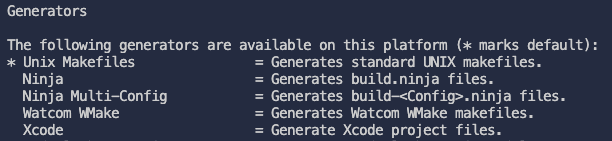
\includegraphics[width=\textwidth]{cmake_generators.png}
	\caption{Ausschnitt einer Liste von verfügbaren Generatoren.}
	\label{fig:cmake_generators}
\end{figure}

Ein wesentlicher Vorteil von CMake liegt in der Trennung von Quell- und Build-Verzeichnissen, was sogenannte Out-of-Source-Builds ermöglicht.
Diese Vorgehensweise trägt zur Schaffung einer übersichtlichen Projektstruktur bei und vereinfacht die Verwaltung von Build-Artefakten.
Zusätlich fördert CMake die hierarchische Strukturierung von Projekten mittels der Implementierung von modularen CMakeLists.txt-Dateien in Unterverzeichnissen.
Dieser Ansatz steigert die Wartbarkeit und Skalierbarkeit komplexer Softwareprojekte.

\subsection*{Make und Makefiles}

% TODO: Build: unklar ob der rein soll; muss noch überarbeitet werden.
%\subsection*{Build}
%Der Begriff Build bezeichnet in der Softwareentwicklung den Prozess, bei dem aus dem Quellcode eines Projekts ein ausführbares Programm, eine Bibliothek oder ein anderes Binärartefakt erzeugt wird. Dieser Vorgang umfasst typischerweise mehrere aufeinanderfolgende Schritte wie Kompilierung, Assemblierung, Verlinkung und optional zusätzliche Nachbearbeitungen wie das Erzeugen von Binär- oder Hex-Dateien für Embedded-Systeme.
%
%Der Build-Prozess wird in der Regel durch ein Build-System automatisiert, das die notwendigen Abhängigkeiten zwischen den Quelldateien verwaltet und auf Änderungen reagiert. Werkzeuge wie make, ninja oder cmake generieren und steuern diesen Prozess, wobei sogenannte Build-Skripte oder Makefiles die Regeln und Schritte definieren. In modernen Entwicklungsumgebungen ist der Build-Prozess oft vollständig integriert und wird durch einen einzigen Befehl oder Mausklick ausgelöst.
%
%Im Kontext der Embedded-Entwicklung besteht ein vollständiger Build-Prozess häufig aus:
%
%dem Übersetzen der Quellcodes (*.c, .cpp) in Objektdateien (.o),
%
%dem Verlinken dieser Objektdateien zu einem ausführbaren Programm (z. B. *.elf),
%
%dem Erzeugen einer herunterladbaren Binär- oder Hex-Datei (z. B. *.bin, *.hex),
%
%sowie optionalen Schritten wie der Speicheranalyse oder der automatisierten Codeprüfung.
%
%Build-Prozesse können zusätzlich durch sogenannte Build-Konfigurationen beeinflusst werden, etwa zur Unterscheidung von Debug- und Release-Versionen mit unterschiedlichen Optimierungs- und Diagnoseoptionen.
%
%Ein effizient organisierter Build-Prozess ist entscheidend für die Wiederholbarkeit, Wartbarkeit und Skalierbarkeit von Softwareprojekten und bildet die Grundlage für weiterführende Konzepte wie Continuous Integration (CI) und automatisiertes Testen.



% TODO: Bis jetzt unklar was hier reingeschrieben werden soll;
\section{Hintergrundwissen}
C++

Assembler

Hochsprache

Hochsprache vs. Assembler/Maschinencode
































